\chapter{He Made \$7M/Year And Paid Zero Taxes}

This chapter follows the School of Hard Knocks interview with Carlton Dennis, curated by LazyingArt LLC through Video2Book. The episode is built around a puzzle: a visibly high-income business owner claims extremely low tax payments, then explains that result through a sequence of mechanisms rather than one hidden trick. We will keep the claims source-conscious, treat the arithmetic as worked examples from the interview, and separate the anecdote, the tax claim, and the mechanism each time they appear.

\section{The Claim That Creates the Puzzle}

The opening is designed to make the reader stop. Carlton is first seen through the viral Ferrari clip: he says he owns a consulting firm, has been an entrepreneur for six years, and made just over \$7.1 million in a single year. Then comes the sharper claim. He says he had already offset his taxes for the year and bought the Ferrari in cash.

The longer interview does not soften that claim. It makes the numbers more explicit. Carlton says that in 2023 he made about \$7.1 million, paid \$0 in federal taxes, and paid \$26,000 in state taxes. He then says that in 2024 the company had crossed \$11.5 million and was on pace to pay less than \$92,000 in total taxes.

\begin{align}
I_{2023} &\approx \$7.1\text{ million},\\
T_{\mathrm{fed},2023} &= \$0,\\
T_{\mathrm{state},2023} &= \$26{,}000,\\
I_{2024} &> \$11.5\text{ million},\\
T_{\mathrm{total},2024} &< \$92{,}000.
\end{align}

These equations are not offered here as verified tax conclusions. They are the numerical form of the interview's central puzzle. The whole lecture turns on the question of how a large income number can coexist with a small reported tax number.

\subsection{Question \& Answer}

\paragraph{Question.}
How can a high-income business owner claim near-zero federal tax liability and still insist that the strategy is legal?

\paragraph{Answer.}
Carlton's answer is that the result is not one magic loophole. He names three recurring mechanisms: income shifting, depreciation through real estate, and philanthropic structure through a private family foundation. In his framing, the tax bill changes because the return is changed by deductions, paper losses, and legal structures that alter taxable income.

\section{Three Mechanisms, Not One Trick}

The host asks directly whether this is legal. Carlton answers directly: everything he is doing, he says, is by the book. That answer matters because it controls the tone of the rest of the chapter. We are not studying a vague promise to ``avoid taxes.'' We are tracking the sequence of mechanisms he claims to use.

He gives three broad categories:

\begin{enumerate}
\item income shifting strategies, which he describes as taking money off the tax return;
\item depreciation, especially paper losses created through real estate;
\item philanthropy through a private family foundation.
\end{enumerate}

The mathematical distinction that appears again and again is the difference between losing cash and recording a loss. A cash loss means money has actually disappeared from the owner's pocket. A paper loss, in Carlton's use here, is a tax loss created by depreciation or similar accounting treatment. The asset may still be owned. The return records a deduction.

A first schematic equation is therefore:

\begin{equation}
I_{\mathrm{taxable}}
\approx
I_{\mathrm{reported}}
-
L_{\mathrm{paper}}
-
D_{\mathrm{other}},
\end{equation}

where \(I_{\mathrm{reported}}\) is income before the discussed offsets, \(L_{\mathrm{paper}}\) is a depreciation-driven paper loss, and \(D_{\mathrm{other}}\) denotes other deductions or structures mentioned in the interview. This is only a model of the interview's reasoning, but it is the right model for the narrative: income appears first, then the chapter asks what can legally reduce it.

\section{Short-Term Rentals As Active Loss Machinery}

The first concrete strategy is real estate, and more precisely short-term rentals. Carlton says that for a full-time W-2 or 1099 taxpayer, short-term rentals are worth studying because the rental can become an active business in his account if the taxpayer manages it and if the tenant stays are short enough. He gives two practical conditions: tenants stay seven days or less, and the taxpayer manages the property for 100 hours.

The spoken mechanism can be written as a chain:

\begin{align}
\mathrm{STR} &: \text{ tenant stays of }7\text{ days or less},\\
H_{\mathrm{management}} &\approx 100\text{ hours},\\
\text{active treatment} &\Longrightarrow \text{cost segregation can matter},\\
\text{cost segregation} &\Longrightarrow \text{accelerated depreciation},\\
\text{accelerated depreciation} &\Longrightarrow L_{\mathrm{paper}}.
\end{align}

The point of this section is not yet the final arithmetic. It is the first bridge from the headline puzzle to an operating rule. If the property can be treated as an active business in the way Carlton describes, then depreciation does not merely sit inside a passive real estate column. It becomes, in the example, a possible offset against W-2 or 1099 income.

The host then slows the discussion down. What about a person who is just starting to make real money, perhaps the first \$100,000, and does not yet have the capital to buy real estate? The lecture now steps backward from advanced real estate strategy to entity structure.

\subsection{Question \& Answer}

\paragraph{Question.}
What if the beginner cannot yet afford the real estate strategy?

\paragraph{Answer.}
Carlton's first answer is entity structuring. He says many self-employed people begin as sole proprietors or single-member entities. That may be acceptable early, but he recommends reviewing the structure once income or profit crosses roughly \$50,000 to \$60,000. At that point, he says, an S corporation may reduce exposure to self-employment tax by separating salary from remaining business profit.

\begin{align}
t_{\mathrm{SE}} &= 15.3\%,\\
\text{review threshold} &\approx \$50{,}000\text{--}\$60{,}000,\\
\text{S corporation pattern} &: \text{ salary }+\text{ remaining profit}.
\end{align}

Carlton then adds a second beginner move: identify expenses that were really business expenses but were paid personally or forgotten. He names phones, laptops, and travel as examples. The rhythm is practical: before the complex strategy, clean up the basic structure; before the large paper loss, make sure ordinary business expenses have not been missed.

\section{Speed, Documentation, And Audit Defense}

The host next asks about the difference between middle-class and wealthy approaches to taxes. Carlton's answer is one word repeated for emphasis: speed. In his description, wealthy clients ask where to move money, when to set up the foundation, and where to send the wire. Less experienced clients hesitate, research endlessly, and may miss the window to act.

But the next anecdote makes clear that speed alone is not enough. Carlton describes a woman who came to him during an IRS audit after seven CPA firms had declined the matter. The disputed deduction was a \$1 million vehicle. The vehicle, she says, was a yacht. Carlton asks why a yacht would be a business purchase. Her answer is the business-purpose story: she is a real estate agent, appears around million-dollar listings, and uses the yacht to show athletes and entertainers what coastal property looks like from the water.

The audit defense depends on evidence. Carlton mentions a captain's log, photos, and expenses from the profit-and-loss statement. He says they used the rule that a business deduction must be ordinary, necessary, and reasonable in pursuit of income. The transcript gives the citation as code section 162A; the common reference is Section 162(a), so the citation should be treated cautiously. The substance of the rule, as presented in the interview, is this:

\begin{equation}
\text{defensible deduction}
\Longleftarrow
\text{business purpose}
+
\text{ordinary and necessary fit}
+
\text{records}.
\end{equation}

This story has an important job in the chapter. It prevents the reader from hearing only bravado. A deduction is not just a number placed on a return. In the story, the deduction has to survive a question: why does this expense belong to this business?

\section{Cars, Depreciation, And Reinvestment}

The interview then moves outside to the cars. At first the scene looks like lifestyle content: Ferrari, G-Wagon, Lamborghini. But the discussion immediately turns those objects into arithmetic. Carlton agrees that cars depreciate. He does not deny the ordinary warning. He changes the frame: depreciation can be a tax event, and the tax effect can become capital to redeploy.

He says he took 100\% bonus depreciation on a car and saved about \$92,000 in taxes. That saving, he says, was reinvested into a Texas multifamily property producing about \$1,400 per month in cash flow.

\begin{align}
S_{\mathrm{tax}} &\approx \$92{,}000,\\
S_{\mathrm{tax}} &\longrightarrow \text{multifamily reinvestment},\\
C_{\mathrm{monthly}} &\approx \$1{,}400/\text{month}.
\end{align}

Then the G-Wagon becomes a more explicit rule example. Carlton says the vehicle qualifies because its gross vehicle weight rating is over 6,000 pounds and because it is used more than 50\% for business. He names Section 179 and Section 168(k). He also states the timing as it stood in the interview: 100\% bonus depreciation in 2022, 80\% in 2023, and 60\% in 2024, with a possible future return to 100\% discussed as speculation.

\begin{align}
\mathrm{GVWR} &> 6{,}000\ \mathrm{lb},\\
u_{\mathrm{business}} &> 50\%,\\
\text{deduction route} &\sim \S 179+\S 168(k).
\end{align}

The host then asks the practical version: how does someone afford a G-Wagon? Carlton answers with a leverage example. Suppose a business owner makes \$200,000, puts \$20,000 down on a qualifying vehicle, and claims a roughly \$200,000 write-off. If the avoided tax bill is roughly \$50,000, the example leaves a claimed cash delta:

\begin{align}
I &= \$200{,}000,\\
W_{\mathrm{vehicle}} &\approx \$200{,}000,\\
T_{\mathrm{avoided}} &\approx \$50{,}000,\\
D_{\mathrm{cash}} &= \$20{,}000,\\
\Delta
&= T_{\mathrm{avoided}}-D_{\mathrm{cash}}\\
&= \$50{,}000-\$20{,}000\\
&= \$30{,}000.
\end{align}

In the interview's logic, \(\Delta\) can go into a cash-flowing asset or back into the business. The car still depreciates. The commercial claim is that depreciation, tax savings, and leverage can be arranged so the owner keeps more deployable capital.

\section{Leverage As Buying Power}

Once the car example is on the table, the host asks the larger debt question: good debt versus bad debt. Carlton distinguishes consumer debt, credit-card debt, and high-interest debt from asset-backed debt. Real estate is his preferred example because it can appreciate, produce income, and support refinancing or a HELOC.

The chapter's compact rule is:

\begin{equation}
\text{buying power}
\quad\text{increases when}\quad
\text{retained cash}
+
\text{credit access}
\quad\text{increase together}.
\end{equation}

This is where the lecture moves from a tax conversation into a wealth-building conversation. Carlton says wealthy families often build portfolios by using debt, reinvesting into real estate, and eventually passing assets to heirs. He also says access to debt grows through banking relationships: use credit, build deposits, earn a private banking relationship, and let the banker understand the business model.

That prepares the final whiteboard calculation. The example will not require the taxpayer to have the full purchase price in cash. It will require control: enough cash for the down payment and enough credit to finance the rest.

\section{Whiteboard Walkthrough: Turning \$500,000 Into A Paper Loss}

The host asks for a specific strategy for someone making \$100,000 a year. Carlton accepts the number and broadens it: this could be W-2 income, 1099 income, or entrepreneurial income. Then he goes to the board.

\begin{figure}
\centering

\includegraphics[width=\linewidth]{lecture_04_figure_02.png}
\caption{The short-term rental walkthrough on the whiteboard. The visible notes include \(\mathrm{STR}=7\) days or less, a 100-hour management note, the \$500,000 property example, and a partially visible cost segregation line.}
\label{fig:str-board}
\end{figure}

The board frame matters because it shows the lecture turning into a calculation. Some of the writing is obscured by the speakers and microphone, so the clean reconstruction below follows the transcript where the frame is incomplete.

Start with income:

\begin{equation}
I=\$100{,}000.
\end{equation}

Now introduce the property and financing:

\begin{align}
P &= \$500{,}000,\\
D &= \$100{,}000,\\
L &= P-D\\
  &= \$500{,}000-\$100{,}000\\
  &= \$400{,}000.
\end{align}

Here \(P\) is the property price, \(D\) is the cash saved for the purchase, and \(L\) is the loan. This is the leverage point: the taxpayer controls a \$500,000 asset without having \$500,000 in cash.

Next come the short-term rental conditions visible on the board:

\begin{align}
\mathrm{STR} &= 7\text{ days or less},\\
H_{\mathrm{management}} &= 100\text{ hours}.
\end{align}

Carlton then says that a cost segregation study can produce, on average in this example, a year-one write-off equal to 20\% of the building's purchase price. The 20\% term is transcript-supported rather than clearly visible in the frame, so the reconstruction should be read as the spoken calculation paired with the board evidence.

\begin{align}
L_{\mathrm{paper}}
&\approx 20\%\times P\\
&=0.20\times \$500{,}000\\
&=\$100{,}000.
\end{align}

Now the example closes:

\begin{align}
I_{\mathrm{taxable}}
&\approx I-L_{\mathrm{paper}}\\
&=\$100{,}000-\$100{,}000\\
&\approx \$0.
\end{align}

This is the lecture's most explicit mathematical payoff. The claim is not that the property lost \$100,000 of cash value. The claim is that depreciation creates a paper loss large enough, in the example, to offset the \$100,000 of income.

\begin{figure}
\centering
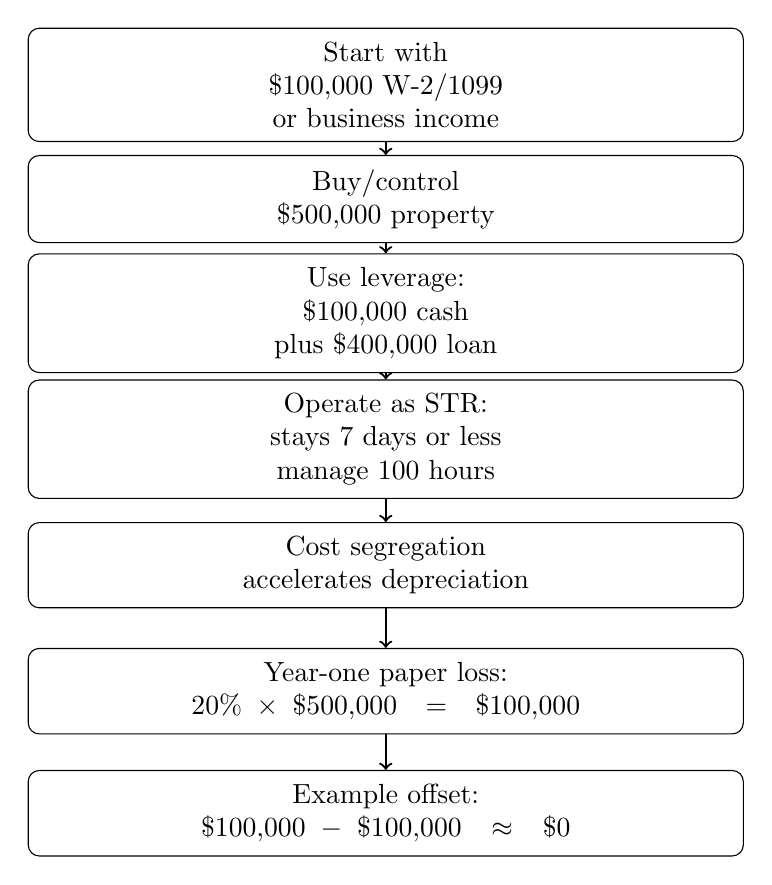
\begin{tikzpicture}[
  every node/.style={draw, rounded corners, align=center, text width=0.72\linewidth, inner sep=5pt},
  arrow/.style={->, thick}
]
\node (a) at (0,0) {Start with\\ \(\$100{,}000\) W-2/1099\\ or business income};
\node (b) at (0,-1.45) {Buy/control\\ \(\$500{,}000\) property};
\node (c) at (0,-2.90) {Use leverage:\\ \(\$100{,}000\) cash\\ plus \(\$400{,}000\) loan};
\node (d) at (0,-4.50) {Operate as STR:\\ stays \(7\) days or less\\ manage \(100\) hours};
\node (e) at (0,-6.10) {Cost segregation\\ accelerates depreciation};
\node (f) at (0,-7.70) {Year-one paper loss:\\ \(20\%\times \$500{,}000=\$100{,}000\)};
\node (g) at (0,-9.25) {Example offset:\\ \(\$100{,}000-\$100{,}000\approx \$0\)};

\draw[arrow] (a) -- (b);
\draw[arrow] (b) -- (c);
\draw[arrow] (c) -- (d);
\draw[arrow] (d) -- (e);
\draw[arrow] (e) -- (f);
\draw[arrow] (f) -- (g);
\end{tikzpicture}
\caption{A narrow reconstruction of the short-term rental and cost-segregation mechanism. The original board frame remains nearby because it is the visual evidence for the conditions and setup.}
\label{fig:str-flow}
\end{figure}

Carlton then scales the intuition. If the income were \$1 million, he says, one would need a larger property or larger set of properties. This is why he returns to debt: the method depends on control over enough depreciable asset value to produce a large enough paper loss.

The final tax tactic is the Augusta rule. Carlton describes its origin in short-term rentals around the Masters golf tournament in Augusta, Georgia, then says that federal tax code allows a primary residence to be rented for 14 days or less without tax on that rental income. For business owners, he describes an S corporation renting the owner's primary residence for meetings, deducting the rent, and sending rent back to the individual.

\begin{equation}
\text{primary-residence rental days}\leq 14
\quad\Longrightarrow\quad
\text{rental income excluded, as described by Carlton}.
\end{equation}

That final rule is a closing example, not a second main derivation. The lecture has already spent its energy on the worked short-term rental calculation.

\section{Summary}

The interview begins with a status object, but the chapter's real object is an equation:

\begin{equation}
\text{taxable income in the example}
\approx
\text{income}
-
\text{documented deductions}
-
\text{paper losses}.
\end{equation}

Carlton's claimed mechanisms arrive in a deliberate order. First come the headline numbers and the legality question. Then come the three broad categories: income shifting, depreciation, and foundation giving. The practical path narrows into short-term rentals, entity structure, ordinary business write-offs, audit documentation, vehicle depreciation, reinvestment, leverage, banking relationships, and finally the whiteboard example.

The most concrete calculation is the \$500,000 property walkthrough: \$100,000 of income, \$100,000 of cash, \$400,000 of debt, short-term rental treatment, 100 hours of management, cost segregation, and a claimed \$100,000 paper loss. The lasting lesson for the broader book is not that every reader can copy the same tax result. It is that wealth in this interview is presented as control over structures: entities, assets, timing, records, debt, and the rules that determine what income finally becomes taxable.